\documentclass[portrait]{seminar}
%\usepackage{pandora}
\usepackage{color}
\usepackage{fancybox}
\usepackage{alltt}
\usepackage{epsfig}
\usepackage{rail}
\usepackage{bar}
\usepackage{url}
\usepackage{rotating}
\usepackage[normalem]{ulem}
\usepackage{latexsym}
\usepackage{amsmath}

\begin{document}

\boldmath
\newcommand{\RA}{$\rightarrow$}
\newcommand{\LL}{\mbox{$[$\hspace{-0.15em}$[$}}
\newcommand{\RR}{\mbox{$]$\hspace{-0.15em}$]$}}
\newcommand{\CC}[1]{\mbox{\tt $\LL$#1$\RR$}}

\slideframe{shadow}

%%% Activate one of these to get either Aarhus style or McGill style 
%%% by putting a #1 in the appropriate line.
\newcommand{\mcgill}[1]{#1}
\newcommand{\aarhus}[1]{}

%%% Define this to be the name of your term
\newcommand{\courseterm}{Fall 2012}




\aarhus{
\newpagestyle{dOvsstyle}{dOvs'98 Week 38 \hfil The JOOS language}{\hfil \thepage}
}

\mcgill{
\newpagestyle{dOvsstyle}{ COMP 520 \courseterm  \hfil The JOOS language (\thepage)}{}
}

\slidepagestyle{dOvsstyle}

\begin{slide*}
\begin{tabbing}
\aarhus{{\Large\bf Week 38}\\}
~\\
{\Huge\bf The}\\ ~\\\psfig{file=joos.EPSF,width=4cm}\\ ~\\{\Huge\bf language}\\
\end{tabbing}
\vfil
\end{slide*}

\begin{slide*}
The Java language:
\begin{itemize}
\item was originally called Oak;
\item was developed as a small, clean, OO language for programming
     consumer devices;
\item was built into the Webrunner browser;
\item matured into Java and HotJava;
\item is now supported by many browsers, allowing Java programs
     to be embedded in WWW pages;
\item is also used by web servers, even if the client user is not running
  Java; and
\item is the implementation language for several large applications.
\end{itemize}
\vfil
\end{slide*}

\begin{slide*}
Basic compilation ({\tt .java} $\rightarrow$ {\tt .class}):
\begin{itemize}
\item Java programs are developed as source code for a collection of Java classes;
\item each class is compiled into Java Virtual Machine (JVM) bytecode;
\item bytecode is interpreted or JIT-compiled using some implementation of the JVM;
\item Java supports a GUI; and
\item many browsers have Java plugins for executing JVM bytecode.
\end{itemize}
\vfil
\end{slide*}

\def\C++{\leavevmode\rm{\hbox{C\hskip -0.1ex\raise 0.25ex\hbox{\small ++}}}}
\begin{slide*}
Major benefits of Java:
\begin{itemize}
\item it's object-oriented;
\item it's a ``cleaner'' OO language than \C++{};
\item it's portable (except for native code);
\item it's distributed and multithreaded;
\item it's secure;
\item it supports windowing and applets;
\item it's semantics is completely standardized;
\item it has a huge class library; and
\item it's finally finally finally officially open source.
\end{itemize}
\vfil
\end{slide*}

\begin{slide*}
Java security has many sources:
\begin{itemize}
\item programs are strongly type-checked at compile-time;
\item array bounds are checked at run-time;
\item {\tt null} pointers are checked at run-time;
\item there are no explicit pointers;
\item dynamic linking is checked at run-time; and
\item class files are verified at load-time.
\end{itemize}
\vfil
\end{slide*}

\begin{slide*}
Major drawbacks of Java:
\begin{itemize}
\item it misses some language features, e.g. genericity (until 1.5),
  multiple inheritance, operator overloading;
\item it does not have one {\em single} standard ({\tt JDK 1.0.2} vs.\ {\tt JDK
    1.1.*} vs.\ \ldots) and probably never will; 
\item it can be slower than C++ for expensive numeric computations due to
dynamic array-bounds checks;~~ $Z^{\displaystyle Z^{\displaystyle
Z^{\displaystyle ZZ}}}$~~ and
\item it's not JOOS.
\end{itemize}
\vfil
\end{slide*}

\begin{slide*}
Goals in the design of JOOS:
\begin{itemize}
\item extract the object-oriented essence of Java;
\item make the language small enough for course work, yet
  large enough to be interesting;
\item provide a mechanism to link to existing Java code; and
\item ensure that every JOOS program is a valid Java program, such
  that JOOS is a strict subset of Java.
\end{itemize}
\vfil
\end{slide*}

\begin{slide*}
Programming in JOOS:
\begin{itemize}
\item each JOOS program is a collection of classes;
\item there are ordinary classes which are used to
      develop JOOS code; and
\item there are external classes which are used to
      interface to Java libraries.
\end{itemize}

\vspace{0.1in}

An ordinary class consists of:
\begin{itemize}
\item protected fields;
\item constructors; and
\item public methods.
\end{itemize}
\vfil
\end{slide*}

\begin{slide*}
\begin{scriptsize}
\begin{verbatim}
$ cat Cons.java
public class Cons {
  protected Object first;
  protected Cons rest;
 
  public Cons(Object f, Cons r) 
  { super(); first = f; rest = r; }
 
  public void setFirst(Object newfirst) 
  { first = newfirst; }
 
  public Object getFirst() 
  { return first; }
 
  public Cons getRest()
  { return rest; }
 
  public boolean member(Object item)
  { if (first.equals(item))
       return true;
    else if (rest==null)
       return false;
    else
       return rest.member(item);
  }
 
  public String toString()
  { if (rest==null)
       return first.toString();
    else
       return first + " " + rest;
  }
}
\end{verbatim}
\end{scriptsize}
\vfil
\end{slide*}

\begin{slide*}
Notes on the {\tt Cons} example:
\begin{itemize}
\item fields in JOOS must be {\em protected}: they can only be accessed via
objects of the class or its subclasses;
\item constructors in JOOS must start by
invoking a constructor of the superclass, i.e. by calling {\tt
  super(...)} where the argument types determine the constructor called;
\item methods in JOOS must be {\em public}: they can be invoked by any object; and
\item only constructors in JOOS can be overloaded, other methods
  cannot.
\end{itemize}
\vfil
\end{slide*}

\begin{slide*}
Other important things to note about JOOS:
\begin{itemize}
  \item subclassing must not change the signature of a method;
  \item local declarations must come at the beginning of the statement sequence
  in a block; and
  \item every path through a non-void method must return a value. (In Java such
  methods can also throw exceptions.)
\end{itemize}
\vfil
\end{slide*}

\begin{slide*}
The class hierarchies in JOOS and Java are both single inheritance,
i.e.\ each class has exactly one superclass, except for the root class:

\begin{center}
\setlength{\unitlength}{0.0005in}%
%
\begingroup\makeatletter\ifx\SetFigFont\undefined%
\gdef\SetFigFont#1#2#3#4#5{%
  \reset@font\fontsize{#1}{#2pt}%
  \fontfamily{#3}\fontseries{#4}\fontshape{#5}%
  \selectfont}%
\fi\endgroup%
\begin{picture}(4824,3924)(589,-4873)
\thicklines
\put(2701,-1261){\framebox(600,300){}}
\put(3001,-1261){\line(-5,-2){1500}}
\put(1201,-2161){\framebox(600,300){}}
\put(2101,-2161){\framebox(600,300){}}
\put(3301,-2161){\framebox(600,300){}}
\put(3001,-1261){\line(-1,-1){600}}
\put(3001,-1261){\line( 1,-1){600}}
\put(3601,-2161){\line( 0,-1){600}}
\put(1801,-3061){\framebox(600,300){}}
\put(601,-3061){\framebox(600,300){}}
\put(1501,-2161){\line(-1,-1){600}}
\put(1501,-2161){\line( 1,-1){600}}
\put(3301,-3061){\framebox(600,300){}}
\put(2851,-3961){\framebox(600,300){}}
\put(3751,-3961){\framebox(600,300){}}
\put(3601,-3061){\line(-5,-2){1500}}
\put(3601,-3061){\line(-3,-4){450}}
\put(3601,-3061){\line( 3,-4){450}}
\put(3601,-3061){\line( 5,-2){1500}}
\put(1801,-3961){\framebox(600,300){}}
\put(4801,-3961){\framebox(600,300){}}
\put(3151,-3961){\line( 0,-1){600}}
\put(2851,-4861){\framebox(600,300){}}
\end{picture}
\end{center}

The root class is called {\tt Object}, and any class
without an explicit {\tt extends} clause is a subclass of {\tt Object}.
\vfil
\end{slide*}
 
\begin{slide*}
The definition of {\tt Cons} is equivalent to:

\begin{scriptsize}
\begin{verbatim}

public class Cons extends Object
{ ... }

\end{verbatim}
\end{scriptsize}

which gives the tiny hierarchy:\\

\begin{scriptsize}
\begin{center}
\begin{tabular}{|l|}
\hline
{\tt Object}\\\hline
{\tt public String toString();}\\
{\tt public boolean equals(Object obj);}\\\hline
\end{tabular}\\
\rule{3pt}{4ex}\\
\begin{tabular}{|l|}
\hline
{\tt Cons}\\\hline
{\tt public void setFirst(Object newfirst);}\\
{\tt public Object getFirst();}\\
{\tt public Cons getRest();}\\
{\tt public boolean member(Object item);}\\
{\tt public String toString();}\\\hline
\end{tabular}
\end{center}
\end{scriptsize}

\vfil
\end{slide*}

\begin{slide*}
The class {\tt Object} has two methods:
\begin{itemize}
\item {\tt toString()} returns a string encoding the type and object id; and
\item {\tt equals()} returns true if the object reference denotes the current object.
\end{itemize}

\vspace{0.1in}

These methods are often overridden in subclasses:
\begin{itemize}
\item {\tt toString()} encodes the value as a string; and
\item {\tt equals()} decides a more abstract equality.
\end{itemize}

\vspace{0.1in}

When overriding a method, the argument types and return types must remain
the same.

\vspace{0.1in}

When overriding {\tt equals()}, {\tt hashcode()} must also be
overridden: equal objects {\em must} produce the same hashcode.
\vfil
\end{slide*}

\begin{slide*}
Extending the {\tt Cons} class:\\

\begin{scriptsize}
\begin{verbatim}
$ cat ExtCons.java
public class ExtCons extends Cons {
  protected int intField;
 
  public ExtCons(Object f, Cons r, int i)
  { super(f,r);
    intField = i;
  }
 
  public void setIntField(int i)
  { intField = i; }
 
  public int getIntField()
  { return(intField); }
}
\end{verbatim}
\end{scriptsize}
\vfil
\end{slide*}

\begin{slide*}
The extended hierarchy:\\

\begin{scriptsize}
\begin{center}
\begin{tabular}{|l|}
\hline
{\tt Object}\\\hline
{\tt public String toString();}\\
{\tt public boolean equals(Object obj);}\\\hline
\end{tabular}\\
\rule{3pt}{4ex}\\
\begin{tabular}{|l|}
\hline
{\tt Cons}\\\hline
{\tt public void setFirst(Object newfirst);}\\
{\tt public Object getFirst();}\\
{\tt public Cons getRest();}\\
{\tt public boolean member(Object item);}\\
{\tt public String toString();}\\\hline
\end{tabular}\\
\rule{3pt}{4ex}\\
\begin{tabular}{|l|}
\hline
{\tt ExtCons}\\\hline
{\tt public void setIntField(int i);}\\
{\tt public int getIntField();}\\\hline
\end{tabular}
\end{center}
\end{scriptsize}
\vfil
\end{slide*}

\begin{slide*}
Using the {\tt Cons} class:

\begin{scriptsize}
\begin{verbatim}
$ cat UseCons.java
import joos.lib.*;
 
public class UseCons {
 
  public UseCons() { super(); }
 
  public static void main(String argv[])
    { Cons l;
      JoosIO f;
 
      l = new Cons("a",new Cons("b",new Cons("c",null)));
      f = new JoosIO();
      f.println(l.toString());
      f.println("first is " + l.getFirst());
      f.println("second is " + l.getRest().getFirst());
      f.println("a member? " + l.member("a"));
      f.println("z member? " + l.member("z"));
    }
}
\end{verbatim}
\end{scriptsize}

A Java program (not an applet) requires a {\tt main()} method.

It is necessary to {\tt import} library functions such as {\tt println()}.
\vfil
\end{slide*}

\begin{slide*}
Compile and run the {\tt UseCons} program:
\begin{scriptsize}
\begin{verbatim}
$ javac joos/lib/*.java
$ joosc UseCons.java Cons.java
$ java UseCons
\end{verbatim}
\end{scriptsize}

The {\tt UseCons} program builds these objects:\\

\begin{center}
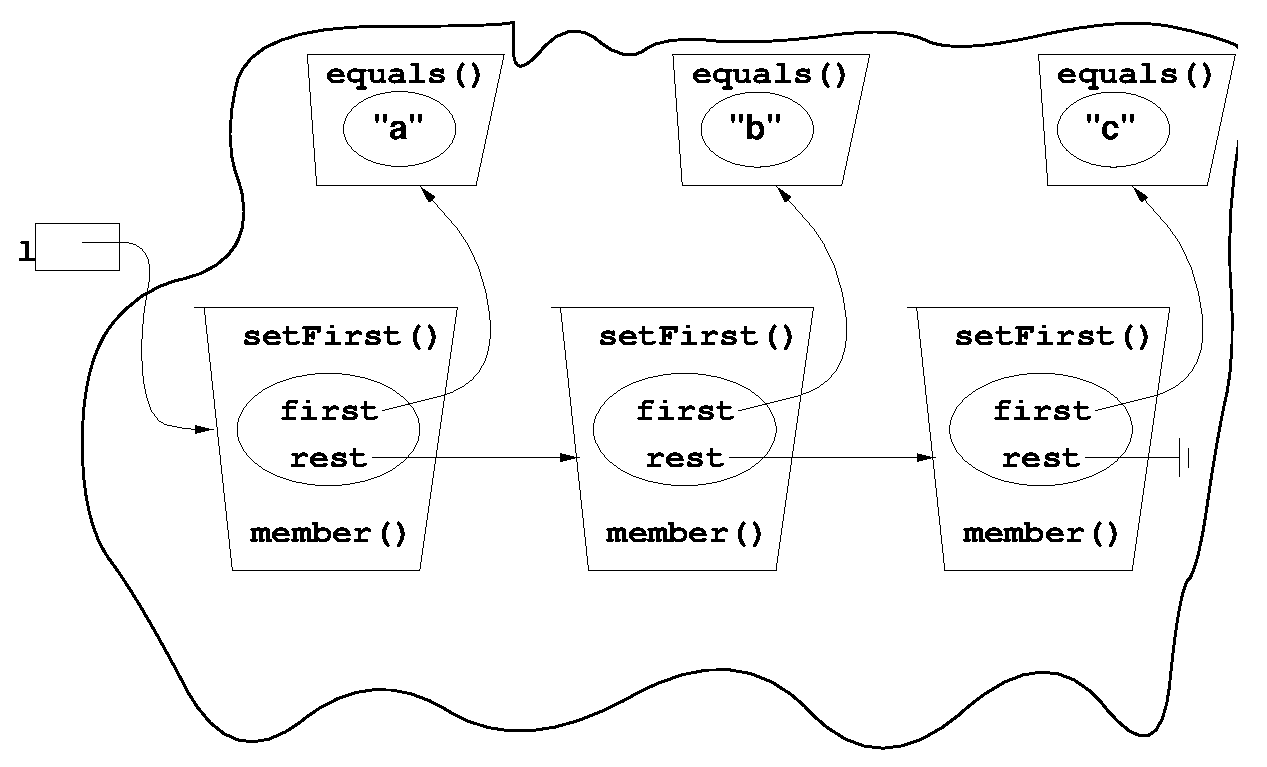
\psfig{file=list.eps, width=16em}
\end{center}

The output of the {\tt UseCons} program is:

\begin{scriptsize}
\begin{verbatim}
a b c
first is a
second is b
a member? true
z member? false
\end{verbatim}
\end{scriptsize}

\vfil
\end{slide*}

\begin{slide*}
Types in JOOS are either primitive types:
\begin{itemize}
\item {\tt boolean}: {\tt true} and {\tt false};
\item {\tt int}: $-2^{31} \ldots 2^{31}-1$;
\item {\tt char}: the ASCII characters;
\end{itemize}
or user-defined class types;

or externally defined class types:
\begin{itemize}
\item {\tt Object};
\item {\tt Boolean};
\item {\tt Integer};
\item {\tt Character};
\item {\tt String};
\item {\tt BitSet};
\item {\tt Vector}; 
\item {\tt Date}.
\end{itemize}

Note that {\tt boolean} and {\tt Boolean} are different.
\vfil
\end{slide*}

\begin{slide*}
Types in Java and JOOS:
\begin{itemize}
\item Java is strongly-typed;
\item
Java uses the name of a class as its type;
\item
given a type of class {\tt C}, any instance
      of class {\tt C} or a subclass of {\tt C} is a permitted value;
\item
there is ``down-casting'' which is automatically checked at
run-time:

\begin{scriptsize}
\begin{verbatim}
SubObject subobj = (SubObject) obj; 
\end{verbatim}
\end{scriptsize}

\item
there is an explicit {\tt instanceof} check:

\begin{scriptsize}
\begin{verbatim}
if (subobj instanceof Object) 
  return true; 
else
  return false;
\end{verbatim}
\end{scriptsize}

\item
and finally some type-checking must be done at run-time.
\end{itemize}
\vfil
\end{slide*}

\begin{slide*}
Statements in JOOS:

\begin{itemize}
\item expression statements:

\begin{scriptsize}
\begin{verbatim}
x = y + z;
x = y = z;
a.toString(l);
new Cons("abc",null);
\end{verbatim}
\end{scriptsize}

\item  block statements:

\begin{scriptsize}
\begin{verbatim}
{ int x;
  x = 3;
}
\end{verbatim}
\end{scriptsize}

\item control structures:

\begin{scriptsize}
\begin{verbatim}
if (l.member("z")) { 
   // do something 
}

while (l != null) { 
   // do something
   l = l.getRest();
}
\end{verbatim}
\end{scriptsize}

\item return statements:

\begin{scriptsize}
\begin{verbatim}
return;

return true;
\end{verbatim}
\end{scriptsize}

\end{itemize}
\vfil
\end{slide*}

\begin{slide*}
Expressions in JOOS:

\begin{itemize}
\item constant expressions:
\begin{scriptsize}
\begin{verbatim}
true, 13, '\n', "abc", null
\end{verbatim}
\end{scriptsize}
\item variable expressions:
\begin{scriptsize}
\begin{verbatim}
i, first, rest
\end{verbatim}
\end{scriptsize}
\item binary operators:
\begin{scriptsize}
\begin{verbatim}
||
&&
!= ==
< > <= >= instanceof
+ -
* / %
\end{verbatim}
\end{scriptsize}
\item unary operators:
\begin{scriptsize}
\begin{verbatim}
-
!
\end{verbatim}
\end{scriptsize}
\end{itemize}
\vfil
\end{slide*}

\begin{slide*}
Expressions in JOOS:

\begin{itemize}
\item class instance creation:
\begin{scriptsize}
\begin{verbatim}
new Cons("abc",null)
\end{verbatim}
\end{scriptsize}
\item cast expressions:
\begin{scriptsize}
\begin{verbatim}
(String) getFirst(list)
(char) 119
\end{verbatim}
\end{scriptsize}
\item method invocation:
\begin{scriptsize}
\begin{verbatim}
l.getFirst()
super.getFirst();
l.getFirst().getFirst();
this.getFirst();
\end{verbatim}
\end{scriptsize}
\end{itemize}
\vfil
\end{slide*}

\begin{slide*}
Abstract methods and classes:
\begin{itemize}
\item a method may be {\tt abstract}, where no implementation is given;
\item if a class contains one or more {\tt abstract} methods, it must be
               defined as an {\tt abstract} class;
\item the constructor of an {\tt abstract} class cannot be invoked;
\item {\tt abstract} classes are used to define ``frameworks''.
\end{itemize}
\vfil
\end{slide*}

\begin{slide*}
\begin{scriptsize}
\begin{verbatim}
$ cat Benchmark.java
import joos.lib.*;
 
public abstract class Benchmark {
 
  protected JoosSystem s;  // JOOS interface to 
                           // the Java System Class
 
  public Benchmark() 
  { super();
    s = new JoosSystem();
  }
 
  // Hook for actual benchmark
  public abstract void benchmark();  
 
  // driver to time repeated executions
  public int myrepeat(int count)     
  { int start;
    int i;
 
    start = s.currentTimeMillis();
    i = 0;
    while (i < count) { 
      this.benchmark();
      i = i+1;
    }
    return s.currentTimeMillis()-start;
  }
}
\end{verbatim}
\end{scriptsize}
\vfil
\end{slide*}

\begin{slide*}
\begin{scriptsize}
\begin{verbatim}
$ cat ExtBenchmark.java
public class ExtBenchmark extends Benchmark {
  public ExtBenchmark() {
    super();
  }
 
  public void benchmark() {}   // timing an empty method
}

$ cat UseBenchmark.java
import joos.lib.*;

public class UseBenchmark {
 
  public UseBenchmark() { super(); }
 
  public static void main(String argv[])
  { ExtBenchmark b;
    JoosIO f;
    int reps;
    int time;

    b = new ExtBenchmark();
    f = new JoosIO();

    f.print("Enter number of repetitions: ");
    reps = f.readInt();
    time = b.myrepeat(reps);
    f.println("time is " + time + " millisecs");
  }
}
\end{verbatim}
\end{scriptsize}
\vfil
\end{slide*}

\begin{slide*}
Final methods and classes:
\begin{itemize}
\item the {\tt final} keyword is used when no modifications to functionality are allowed;
\item a {\tt final} method cannot be overridden by subclasses;
\item a {\tt final} class cannot be extended;
\item {\tt final} classes typically belong to libraries: {\tt Boolean}, {\tt
Integer}, and {\tt String} (for security purposes).
\end{itemize}

\vspace{0.1in}

Note that JOOS does not provide {\tt final} {\em fields} like Java does.

\vfil
\end{slide*}

\begin{slide*}
Synchronized methods:

\begin{itemize}
\item Java and JOOS programs can start multiple threads;
\item sometimes access to a shared resource must be protected, such
  that only one thread is in a {\em critical section} at a time;
\item each object has an associated lock; and
\item JOOS provides {\tt synchronized} methods, such that when a thread invokes a {\tt synchronized}
          method on an object, the thread does not enter the method
          until it has successfully acquired the target object's lock
          and it holds on to the lock until the method execution completes.
\end{itemize}

\vspace{0.1in}

Note that JOOS does not provide {\tt synchronized} blocks like Java does.

\vfil
\end{slide*}

\begin{slide*}
\begin{scriptsize}
\begin{verbatim}
$ cat SyncBox.java
public class SyncBox {
  protected Object boxContents;
 
  public SyncBox() { super(); }
 
  // return contents of the box, set contents to null
  public synchronized Object get()
  { 
    Object contents;
    contents = boxContents;
    boxContents = null;
    return contents;
  }
 
  // put something in the box,
  // if the box already has something in it, return false
  // else fill the box, return true
  public synchronized boolean put (Object contents)
  { 
    if (boxContents != null) return false;
    boxContents = contents;
    return true;
  }
}
\end{verbatim}
\end{scriptsize}
\vfil
\end{slide*}

\begin{slide*}
External classes in Java:
\begin{itemize}
\item Java compiles programs with respect to a set of libraries of precompiled
       class files; and
\item when a Java compiler encounters an unknown method, it searches the precompiled
bytecode for an implementation.
\end{itemize}

External classes in JOOS:
\begin{itemize}
\item JOOS compiles programs with respect to a set of libraries of precompiled
       class files; but
\item external classes must be explicitly presented to the JOOS compiler.
\end{itemize}
\vfil
\end{slide*}

\begin{slide*}
\begin{scriptsize}
\begin{verbatim}
$ cat joos/extern/javalib.joos

[...]

// java.lang.String
extern public final class String in "java.lang" {
  public String();
  public String(String value);
  public String(StringBuffer buffer);
  public String vlaueOf(boolean b);
  public char charAt(int index);
  public int compareTo(String anotherString);
  public boolean endsWith(String suffix);
  public boolean equals(Object obj);
  public boolean equalsIgnoreCase(String anotherString);
  public int indexOf(String str, int fromIndex);
  public int lastIndexOf(String str, int fromIndex);
  public int length();
  public boolean regionMatches(boolean ignoreCase,
      int toffset, String other, int ooffset, int len);
  public boolean startsWith(String prefix, int toffset);
  public String substring(int beginIndex, int endIndex);
  public String concat(String str);
  public String toLowerCase();
  public String toUpperCase();
  public String toString();
  public String trim();
}

[...]
\end{verbatim}
\end{scriptsize}
\vfil
\end{slide*}

\begin{slide*}
External declarations for Java libraries:
\begin{itemize}
\item {\tt javalib.joos}
\item {\tt appletlib.joos}
\item {\tt awtlib.joos}
\item {\tt netlib.joos}
\item {\tt BigDecimal.joos}
\end{itemize}

External declarations for JOOS libraries:
\begin{itemize}
\item {\tt jooslib.joos}
\end{itemize}
\vfil
\end{slide*}

\begin{slide*}
Example JOOS programs:
\begin{itemize}
\item {\tt AppletGraphics}:
simple graphics programs to be displayed via a browser;
\item {\tt AwtDemos}:
 examples of using the Abstract Windows Toolkit;
\item {\tt ImageDemos}:
two techniques for displaying an animation;
\item {\tt Network}:
simple examples of interacting over the network;
\item {\tt Simple}:
a relatively large collection of simple programs;
\item {\tt Threads}: simple multithreaded programs; and
\item {\tt WIGapplets}: examples of WIG applets.
\end{itemize}

\vspace{0.1in}

All examples should work, please email your TA if they do not.

\vfil
\end{slide*}

\begin{slide*}
When compared to Java, JOOS:
\begin{itemize}
\item does not support packages, interfaces, exceptions, some control structures,
mixed statements and declarations;
\item has only {\tt protected} fields and {\tt public} methods;
\item does not allow overloading of methods;
\item does not support arrays;
\item does not allow static methods;
\item supports only {\tt int}, {\tt boolean}, and {\tt char} as primitive types; and
\item uses external class declarations.
\end{itemize}
\vfil
\end{slide*}

\begin{slide*}
Converting between JOOS \& Java source code ({\tt *.java}, {\tt *.joos}), Jasmin
assembler ({\tt *.j}) and Java bytecode ({\tt *.class}):

\begin{center}
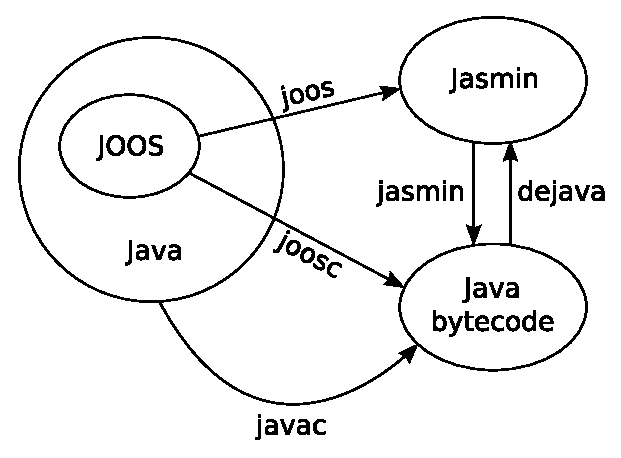
\psfig{file=figs/joos_to_bytecode.eps,width=18em}
\end{center}

{\tt joosc} simply calls {\tt joos} and then {\tt jasmin}.

\vfil
\end{slide*}

\end{document}
